\date{\today}

%\documentclass[journal=jacsat,manuscript=communication,layout=twocolumn]{achemso}
%\documentclass[jctcce,letterpaper,twocolumn,floatfix,preprintnumbers,superscriptaddress]{revtex4}
% \documentclass[12pt,preprint,aps,prb]{revtex4}
% \documentclass[aps,preprint,showpacs,superscriptaddress,groupedaddress]{revtex4}  % for double-spaced preprint
\documentclass[aps,prl,twocolumn,superscriptaddress,groupedaddress]{revtex4}  % for review and submission
\usepackage{dcolumn,graphicx,amsmath,amssymb,algorithm,algpseudocode}
\usepackage{todonotes}
\usepackage{qcircuit}

\newcommand{\total}{\mathrm{d}}
\newcommand{\ud}{\mathrm{d}}
\newcommand{\erf}{\mathrm{erf}}
\newcommand{\erfc}{\mathrm{erfc}}
\newcommand{\diff}[2]{\frac{\ud {#1}}{\ud {#2}}}
\newcommand{\pdiff}[2]{\frac{\partial #1}{\partial #2}}

\begin{document}

\definecolor{brickred}{rgb}{.72,0,0} 

\title{
BMW Quantum Challenge: Optimizing the Production of Test Vehicles
}

\author{Robert M. Parrish}
\email{rob.parrish@qcware.com}
\author{Rachael Al-Saadon}
\affiliation{
QC Ware Corporation, Palo Alto, CA 94301, USA \\
\textbf{QC Ware Corporation Proprietary and Confidential}
}


\begin{abstract} 
A complete and completely classical solution of the industrial challenge problem
is presented.  Additional gains are potentially possible for extended versions
of this problem and/or for similar problems if hybrid quantum/classical
algorithms are considered - we present some ideas along these lines.

% We solved your problem. \\
% Want to know how? \\
% We can do this with quantum too...\\
% Despite apparent classical complexity, this problem is, at present, not suitable for
% the possibility of practical quantum advantage. We demonstrate this pragmatically
% by direct and tight classical solution of the optimization problem as specified
% in the quantum computing challenge (while noting that this problem does not seem
% to exhibit the typical drastic simplification of ``quantum'' formulations of
% standard binary optimization problems throughout the industry). 
\end{abstract}

\maketitle

\section{Results}

The problem statements variously ask for optimization of the constituents of a
set or
``constellation'' of $n_{\mathrm{C}}$ test vehicles, with each test vehicle taken
from a state space of $\sim 469$ binary dimensions called ``features'' (this and other dimensions
quoted below to vary
in future problem sizes), and with each test vehicle 
satisfying hard ``feature-group'' and ``type-build rule'' constraints
corresponding to $\sim 25$ basic test vehicle types. The problem
statement(s), predicated by the hard constraints, specifically ask for
(1) \textbf{SAT:} 
For a given $n_{\mathrm{C}}$, does there exist, for a given set of
$n_{\mathrm{test}} \sim 644$ tests depending through binary expressions on the state
space of each test vehicle, a set of $n_{\mathrm{C}}$ test cars for which the
$n_{\mathrm{test}}$ tests can be separately evaluated, with the caveat 
that there need be $K_I \sim 1-5$ distinct
test vehicles required to satisfy test $I$ for $I \in [0, n_{\mathrm{test}})$?
(2) \textbf{Weighted MAX-SAT:} For a given $n_{\mathrm{C}}$, what is the optimal
constellation of test vehicles such that the weighted sum of satisfied $n_{\mathrm{test}}$
tests, each requiring $K_I$ distinct test vehicles, is maximized? and 
(3) \textbf{Scheduling (not precisely specified):} For a given set of
$n_{\mathrm{test}}$ tests and corresponding set of $n_{\mathrm{C}}$ test
vehicles satisfying said tests including $\{ K_I \}$ multiplicity constraints in
a MAX-SAT formalism of (2), what is the optimal scheduling of said vehicles into 
a test sequence with at most $n_{\mathrm{slot}} \sim 10$ tests performed on
distinct cars in each timeslot and with tests assigned to integer test groups
with definite sorting of test groups within each car?

A specific instance of the problem class described above was provided by BMW.
Taken naively, this problem instance involves binary optimization over a state
space of $\sim 469\times60 = 27540$ binary variables (plus additional state
space variables for scheduling) with hard constraints and fairly generic logical
expressions needed to specify constraints and objective function values.  As
stated by BMW: ``The provided description is based on the actual numbers and
constraints formulated for this model. It, thus, represents the real complexity
arising in a productive setting.''

Within the problem statement document, solutions to the above problems were
attempted using existing industry-standard SAT solvers and constraint
satisfaction solvers. The SAT problem of (1) was easily solved:
``For 100 cars, the problem can be solved in a few seconds. A linear search counting down
from 100 revealed the solution that at least 60 cars are needed to perform all the specified
750 tests.''
However the weighted MAX-SAT problem of (2) was not solvable:
``On the other hand, the MAX-SAT problem was not solvable in a reasonable time with the
chosen approach.''
Additionally, the scheduling problem of (3) was not solvable:
``[O]n the test laptop, the full problem with 700 tests wasn't solvable in less than 24
hours.''

\begin{figure*}[ht]
\begin{center}
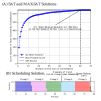
\includegraphics[width=4in]{figures/solution.pdf}
\caption{Characteristics of QC Ware solutions to the ``optimizing the production
of test vehicles'' BMW quantum computing challenge problem. (A) Solutions
to the MAX-SAT, and by corollary, SAT variants of problem variants (2) and (1),
respectively. (B) Solution to the scheduling problem variant (3).}
\label{fig:solution}
\end{center}
\end{figure*}

\textbf{We provide what we believe under the rules of the problem statement
represents a complete and tangible solution to all three specified problems.}
Specifically, we developed a custom C++/Python code library to represent the
details of the problem in a natural format. 
The combination of customized classical solution environment and high
performance implementation allows for very rapid exploration of the
hard-constraint-satisfying parameter space unique to this problem class.  Within
this environment, we developed a powerful and simple set of heuristics to
approximately solve the MAX-SAT variant of the problem. This heuristic MAX-SAT
solver produces nested constellations of test cars with increasing
$n_{\mathrm{C}}$ and concomitant increasing MAX-SAT scores. The MAX-SAT
solutions coming from this heuristic achieve saturation of all specified $644$
tests (including multiplicity considerations) at the same $n_{\mathrm{C}} = 60$
bound determined by standard SAT solvers for problem (1) in the problem
statement document. Thus our MAX-SAT solution provides a tight bound solution
for problem (1) in the process of providing approximate solutions for (2). For
values of $n_{\mathrm{C}} \ll 60$, we believe our heuristic MAX-SAT solutions
are within a few percent of the global optimum. For the scheduling problem of
(3) we develop additional heuristics to schedule the test sequence from the
MAX-SAT optimized constellation fo $n_{\mathrm{C}} = 60$ cars while respecting
the hard constraints of distinct cars within each time slot, strict ordering of
randomly-specified test groups within cars, and separate cars used within the
multiplicity considerations of each test. With the multiplicity considerations
included, there are 766 separate test-car pairs required, mandating a
theoretical floor of 77 test slots. Our heuristic solution provides a nearly
dense scheduling with 78 test slots required, i.e., within 1.3$\%$ of dense
scheduling.

\section{Methods}

\subsection{C++/Python Environment}

To facilitate rapid exploration of the state space for this problem class, we
developed a custom C++11/Python3 library API linked by PyBind11. No additional
dependencies beyond standard C++11, Python3, and the header-only PyBind11 linker
layer are needed - i.e., we do not rely on third-party SAT solvers. This library
contains simple classes enumerating the natural representation of the problem
contents. For instance, a \texttt{SimpleBinaryExpression} class is implemented
to represent the concept of simple all/any binary expressions containing
arbitrary not predicates as encountered throughout the type build rules and the
test rules. Instances of this class store the state of, e.g., a given build rule
predicate or implication expression, and can efficiently check whether this
expression is satisfied for a given proposed vehicle configuration. Two
\texttt{SimpleBinaryExpression} objects are further stacked in a
\texttt{SimpleBinaryImplication} object to represent the predicate and
implication of each type build rule. Multiple \texttt{SimpleBinaryExpression}
objects are chained together in a \texttt{FirstOrderAllBinaryExpression} object
to represent the parenthesized binary expressions present in each test rule.
Additional data structures are constructed to uniquely represent the type
feature groups, the type-specific build rules, the full set of test rules and
corresponding multiplicities, eventually yielding a complete C++ representation
of the full problem. The critical configuration state space of each test vehicle
is efficiently represented by the \texttt{std::vector<bool>} concept, i.e., each
proposed test vehicle is represented by a \texttt{std::vector<bool>} containing the
states of the $\sim 469$ features of each vehicle.
 The entire library is reflexively exposed to Python3 through PyBind11 to merge
the effortless development of Python (i.e., regex for data parsing, short python
scripts to manage various experiments, compile-free debugging through python
printing) with the speed of compiled C++ for rate-limiting operations. The use
of C++ also facilitates the use of single-node parallelism through OpenMP
threading.

\subsection{Test Vehicle Seeds}

One might expect that the guess of $\vec 0$ (i.e., all features turned off)
would yield an acceptable starting guess for a test vehicle configuration.
However, already at $\vec 0$ some of the type build rules are violated, meaning
that $\vec 0$ is outside of the hard constraint space. Moreover, we have
empirically found that some of the $\sim 644$ test rules are rather hard to find
without specific direction within the constraint space. Therefore, to seed a
starting pool of test vehicles, we adopt the following procedure:
\begin{enumerate}
\item For each test rule, we generate a seed test vehicle that satisfies this
test rule with a randomly selected type.
\item To generate this vehicle, we first flip the required features on to
satisfy the test rule. 
\item The active test rule features are then ``masked'' meaning that they are
frozen in current values satisfying the test rule throughout all future steps.
\item In the non-masked features, we then chase constraints until we arrive at a
valid car satisfying the type build rules.
\item If this procedure fails for a given randomly selected type, we randomly
select another type and repeat ad inifitum.
\end{enumerate}
At the end of this procedure we have a pool of $\sim 644$ test vehicles which
are largely ``featureless'' meaning that only the minimal number of features
have been activated to satisfy the test and chase the constraints into the valid
type build rule space. All test rules are present in at least one test vehicle in this
starting pool.

\subsection{MAX-SAT Optimization}

We start from the empty constellation $n_{\mathrm{C}} = 0$. To update this
constellation to $n_{\mathrm{C}} = 1$, we adopt the following procedure:
\begin{enumerate}
\item For each of the $\sim 644$ test vehicles in the the candidate pool, we
perform several tens of thousands of directed Monte Carlo moves designed to
improve the number of rules simultaneously satisfied by the test vehicle, while
respecting the hard constraints. The Monte Carlo moves are described below.
\item We add to the constellation the single car from the updated candidate pool
that maximally increases the number of satisfied tests in the constellation.
\item We update the test set used to direct the Monte Carlo moves in Step 1 to
include only those rules which are unsatisfied by the current constellation.
\item We iterate this procedure until all test rules are satisfied, increasing
the constellation size $n_{\mathrm{C}}$ by one test vehicle per iteration.
\end{enumerate}
At the end of this procedure, we have a set of $n_{\mathrm{C}}$ nested
constellations each of which is a local approximant to the MAX-SAT [Problem (2)]
solution of corresponding constellation size. Once we obtain a constellation
that saturates all tests, we have an upper bound for the SAT solution [Problem
(1)] which turns out to be tight for the specifics of this problem instance.

\subsection{Masked Distance-2 Monte Carlo Moves}

One of the particular specialties of our approach lies in the strength of our
Monte Carlo moves. We adopt the following procedure:
\begin{enumerate}
\item For each test vehicle in the candidate pool, we randomly select two
feature groups to vary.
\item For each of these feature groups we move with equal probability to
deactivate the feature group or to active a random feature index within the
group.
\item We check if the proposed move satisfies the type build rules and return to
1 if not.
\item We check if the proposed move would perturb the masked features discussed
in the previous section, and return to 1 if so. 
\item At this point, we know that the proposed test vehicle is valid and has not
moved a masked feature. If this proposed test vehicle improves the number of
satisfied tests in the active test set, we accept the updated vehicle and return
to 1. Else we reject the proposed test vehicle and return to 1.
\item We loop some user-specified number of iterations, usually on the order of
tens of thousands.
\end{enumerate}

There are several key observations that guided this heuristic choice of Monte
Carlo move scheme:
\begin{itemize}
\item These moves always remain on the constraint space.
\item These moves move by feature group rather than binary variables, and
therefore automatically satisfy the feature group constraint. Direct moves in
binary variables would have vanishing probability of satisfying the feature
group constraints.
\item Distance-2 moves are much more likely to be interesting and valid than
distance-1 moves. E.g., the activation of a single feature group often implies
the activation of another feature group through the type build rules. Such
implications can be satisfied with reasonable probability with distance-2 moves,
but are often unreachable with a sequence of distance-1 moves.
\item The acceptance of moves based on increased test set scores promotes a
compounding improvement of the test vehicle through the iterative procedure.
\end{itemize}

This procedure is implemented within C++, which treats the involved logic almost
natively. As such, we obtain orders of magnitude improvement over a
corresponding Python implementation of this portion of the approach.
Additionally, this stage of the procedure is embarrassingly parallel across the
$\sim 644$ test vehicles in the candidate pool. We parallelize this with OpenMP,
with dynamic scheduling invoked to attempt to load balance across the
anisotropic task sizes encountered.


\subsection{Scheduling}

For scheduling, we were initially considering doing some rather exotic work
involving global optimization, i.e., building a different constellation of test
vehicles that would be more optimized for the scheduling objective function than
for the MAX-SAT objective function. However, we started by exploring an extremely
simple greedy approach involving attempting to schedule our existing SAT/MAX-SAT
constellation of $n_{\mathrm{C}} = 60$ test vehicles, and found that it produced
almost dense packing. Therefore, we will only explain the latter approach here. 

The scheduling heuristic approach works as follows:
\begin{enumerate}
\item We first sort the test rules by test group (first priority) and by
number of required cars for the test (second priority).
\item We traverse the current priority-sorted test set.
\item For each test, we indentify and randomly sort the list of cars which
satisfy the test.
\item For each car in this list, we attempt to add the car to the current time
slot, continuing deeper into the car list if the car already exists in the
current time slot, if the car has already been used previously for this test
(for multi-car tests), or if the car has already been used for a lower-priority
test group. As soon as we find a valid car, we break out of the loop over the
car list.
\item If no test-car pair can be added to the current slot, we ``nuke'' the slot
and kick it onto the schedule with no-ops (i.e., empty time/engineer slots) inside. 
\item If the addition of a car saturates the number of engineer slots, we kick
the slot onto the schedule.
\item We check if the addition of a car saturates a test rule, and update the
test rule set to remove this rule if so.
\item We iterate from 2 until all test rules are satisfied, as evidenced by the
active test set becoming empty.
\end{enumerate}

There is a small chance that this algorithm will enter an infinite loop where a
critical car is greedily used for a lower-priority test, and therefore cannot be
used for a higher-priority test. We have encountered this failure case in only
about 15$\%$ of runs. The existence of even a single successful run producing a
dense schedule obviates this concern. 

Note that we find the absence of specified test groups in the problem
specification to be a major weakness of this part of the challenge. We generated
test groups ranging from 1 to 5 from random integers as sketched in the problem
statement. We did this exactly once using \texttt{numpy.random.randint} and
stored the values in our github repository - i.e., we generated what we feel is
a fair test and then froze it. Note also that we elected to define the priority
order to be sorted from $1$ to $5$ rather than from $5$ to $1$ in the problem
statement for aesthetic reasons - as these values are randomly generated this
makes no difference in problem structure.

\subsection{Feature Groups Collision Issue}

The efficient exploration of the state space in terms of moves in feature groups
requires that the feature groups be disjoint. We found that this was not the
case in the specified problem due to a collision between feature groups 40 and
41. To fix this issue, we modified these two groups and added additional type
build rules to produce an isomorphic variant of the problem with disjoint
feature groups. Details:

Group 40 (28 elements): \texttt{[245, 246, 247, 250, 251, 252, 253, 254, 255,
256, 266, 267, 268, 269, 270, 271, 272, 273, 274, 275, 276, 277, 278, 279, 280,
281, 282, 284]}

Group 41 (46 elements): \texttt{[245, 246, 247, 248, 249, 250, 251, 252, 253,
254, 255, 256, 257, 258, 259, 260, 261, 262, 263, 264, 267, 268, 269, 270, 271,
272, 273, 274, 275, 276, 277, 278, 279, 280, 281, 282, 283, 285, 286, 287, 288,
289, 290, 291, 292, 293]}

Union (48 elements): \texttt{[245, 246, 247, 248, 249, 250, 251, 252, 253, 254,
255, 256, 257, 258, 259, 260, 261, 262, 263, 264, 266, 267, 268, 269, 270, 271,
272, 273, 274, 275, 276, 277, 278, 279, 280, 281, 282, 283, 284, 285, 286, 287,
288, 289, 290, 291, 292, 293]}

Intersection (26 elements): \texttt{[245, 246, 247, 250, 251, 252, 253, 254,
255, 256, 267, 268, 269, 270, 271, 272, 273, 274, 275, 276, 277, 278, 279, 280,
281, 282]}

In Group 40 but not Group 41 (2 elements): \texttt{[266, 284]}

In Group 41 but not Group 40 (20 elements): \texttt{[248, 249, 257, 258, 259,
260, 261, 262, 263, 264, 283, 285, 286, 287, 288, 289, 290, 291, 292, 293]}

This is hugely vexing for efficient enumeration of group-feature-satisfying
vehicle candidates.

This can be overcome by (1) redefining Group 40 to be \texttt{[266, 284]} and
then (2) adding a new global (added for all types) rule to the type build rules:

\texttt{ F266 | F284 => !F245 \& !F246 \& !F247 \& !F250 \& !F251 \& !F252 \& !F253 \&
!F254 \& !F255 \& !F256 \& !F267 \& !F268 \& !F269 \& !F270 \& !F271 \& !F272 \& !F273 \&
!F274 \& !F275 \& !F276 \& !F277 \& !F278 \& !F279 \& !F280 \& !F281 \& !F282}

If the group features are chosen randomly, uniformly, and independently, this
rule has a probability of $2/(1+2)$ to be activated (if 266 xor 284 are true).
The probability of the rule being violated is $\sim 26/(1+46) \sim 0.55$.
Therefore the joint probability of the rule being activated and failing is
$(2/3) * (26/47) \sim 0.37$. Note that this high success probability is somewhat
accidental, and is only due to the fact that the in-40-but-not-in-41 subset is
small relative to the intersection \emph{and} the in-41-but-not-in-40 subset is
large relative to the the intersection. In future, it is recommended that
collisions between feature groups be avoided at all costs in the formulation of
this problem, insofar as is possible.


% \bibliography{jrncodes.bib,refs.bib}
% \bibliographystyle{aip}

\end{document}
